\section{Programming and Configuring the FPGA Device}


The FPGA device must be programmed and configured to implement the designed 
circuit. The required configuration file is generated by the Quartus Prime 
Compiler's Assembler module. Intel's DE-series board allows the configuration to 
be done in two different ways, known as JTAG* and AS modes.
The configuration data is transferred from the host computer (which runs the 
Quartus Prime software) to the board by means of a cable that connects 
a USB port on the host computer to the USB-Blaster connector on the board.
To use this connection, it is necessary to have the USB-Blaster driver 
installed. If this driver is not already installed, consult the 
tutorial {\it Getting Started with Intel's DE-Series Boards}
for information about installing the driver.
Before using the board, make sure that the USB cable is properly connected
and turn on the power supply switch on the board.
 
In the JTAG mode, the configuration data is loaded directly
into the FPGA device. The acronym JTAG stands for Joint Test Action Group. 
This group defined a simple way for testing digital circuits and loading data 
into them, which became an IEEE* standard. If the FPGA is configured in 
this manner, it will retain its 
configuration as long as the power remains turned on. 
The configuration information is lost when the power is turned off.
The second possibility is to use the Active Serial (AS) mode.
In this case, a configuration device that includes some flash memory is used 
to store the configuration data. Quartus Prime software places the configuration 
data into the configuration device on the DE-series board. Then, this data is loaded 
into the FPGA upon power-up or reconfiguration.
Thus, the FPGA need not be configured by the Quartus Prime software if the power 
is turned off and on. 
The choice between the two modes is made by switches on the DE-series 
board. Consult your manual for the location of this switch on your DE-series board. The boards should be set to JTAG mode by default.
This tutorial discusses only the JTAG programming mode.

\subsection{JTAG* Programming for the DE0-CV, DE0-Nano, DE10-Lite, and DE2-115 Boards}

For the DE0-CV, DE0-Nano, DE10-Lite, and DE2-115 Boards, the
programming and configuration task is performed as follows. If using the DE1-SoC board,
then the instructions in the following section should be followed.
To program the FPGA chip, the RUN/PROG switch on the board must be in the RUN position.
Select {\sf Tools $>$ Programmer} to reach the window in Figure~\ref{fig:38}.
Here it is necessary to specify the programming hardware and 
the mode that should be used. If not already chosen by default, 
select JTAG in the Mode box.
Also, if the USB-Blaster is not chosen by default, press the 
{\sf Hardware Setup...} button and select the USB-Blaster in the window
that pops up, as shown in Figure~\ref{fig:39}.

\begin{figure}[H]
   \begin{center}
      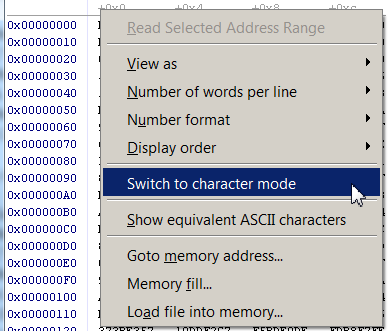
\includegraphics[scale=0.65]{figures/figure38.png}
   \caption{The Programmer window.} 
	 \label{fig:38}
	 \end{center}
\end{figure}

Observe that the configuration file {\it light.sof} is listed in the window in
Figure~\ref{fig:38}. If the file is not already listed, then click {\sf Add File}
and select it.
This is a binary file produced by the Compiler's Assembler module, 
which contains the data needed to configure the FPGA device.
The extension {\it .sof} stands for SRAM Object File.
Ensure the {\sf Program/Configure} check box is ticked, as shown in Figure~\ref{fig:38}.

\begin{figure}[H]
   \begin{center}
      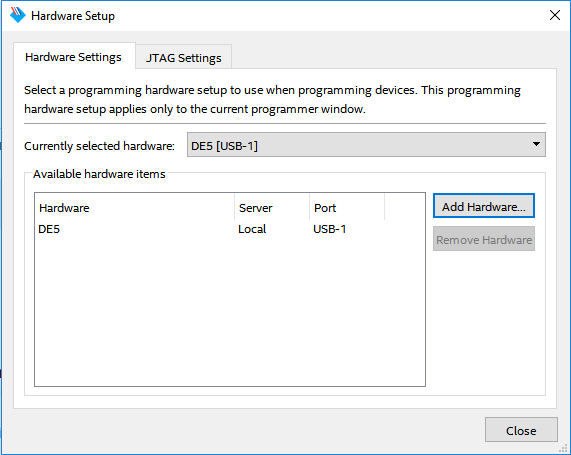
\includegraphics[scale=0.65]{figures/figure39.png}
   \caption{The Hardware Setup window.} 
	 \label{fig:39}
	 \end{center}
\end{figure}

Now, press {\sf Start} in the window in Figure~\ref{fig:38}.
An LED on the board will light up corresponding to the programming operation.
If you see an error reported by Quartus Prime software indicating that
programming failed, then check to ensure that the board is properly powered on.

\subsection{JTAG* Programming for the DE0-Nano-SoC, DE1-SoC Board, DE10-Nano, and DE10-Standard}

For the DE0-Nano-SoC, DE1-SoC Board, DE10-Nano, and DE10-Standard boards, the following steps should be used for programming.
Select {\sf Tools $>$ Programmer} to reach the window in Figure~\ref{fig:SoC1} (if the SOCVHPS device is missing, it can be added through the {\sf Add Device} menu under the \textit{Soc Series V} family).
Here it is necessary to specify the programming hardware and 
the mode that should be used. If not already chosen by default, 
select JTAG in the Mode box.  Also, if {\it DE-SoC} is not chosen by default as the programming
hardware, then press the {\sf Hardware Setup...} button and select the {\it DE-SoC} in the 
window that pops up, as shown in Figure~\ref{fig:SoC2}.

\begin{figure}[H]
   \begin{center}
      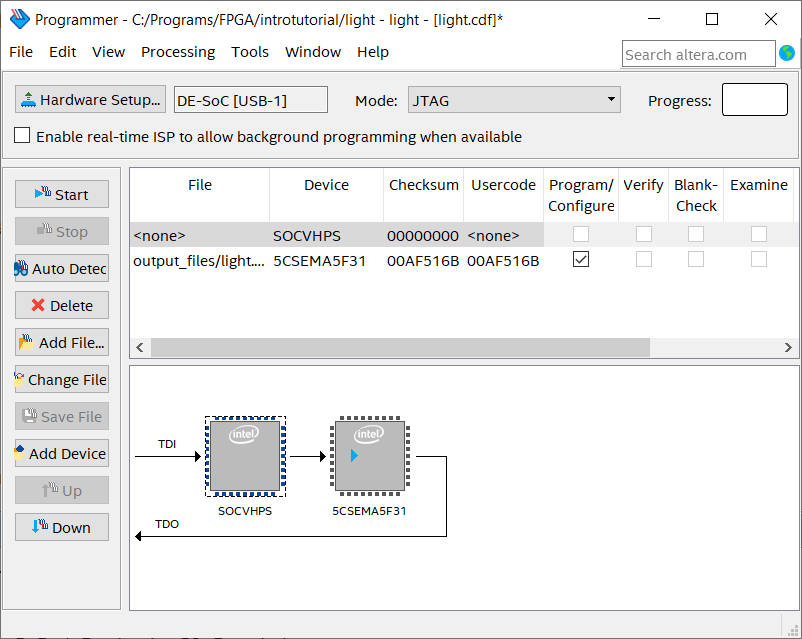
\includegraphics[width=0.75\textwidth]{figures/figureSoC1.png}
   \caption{The Programmer window.} 
	 \label{fig:SoC1}
	 \end{center}
\end{figure}

Observe that the configuration file {\it light.sof} in directory {\it output\_files} is listed in the window in
Figure~\ref{fig:SoC1}. If the file is not already listed, then click {\sf Add File} 
and select it.
This is a binary file produced by the Compiler's Assembler module, 
which contains the data needed to configure the FPGA device.
The extension {\it .sof} stands for SRAM Object File.
Ensure the {\sf Program/Configure} box is checked.
This setting is used to select the FPGA in the Cyclone V SoC chip for programming.
If the {\it SOCVHPS} device is not shown as in Figure~\ref{fig:SoC1}, click {\sf Add Device $>$ SoC Series V $>$ SOCVHPS} then click {\sf OK}.
Ensure that your device order is consistent with Figure~\ref{fig:SoC1} by clicking on a device and then clicking 
\includegraphics[scale=.55]{figures/icon14.png} or 
\includegraphics[scale=.55]{figures/icon13.png}.

\begin{figure}[H]
   \begin{center}
      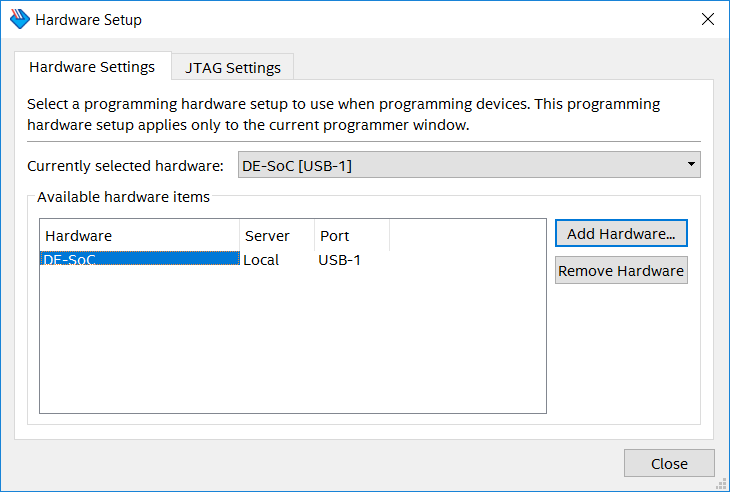
\includegraphics[scale=0.65]{figures/figureSoC2.png}
   \caption{The Hardware Setup window.} 
	 \label{fig:SoC2}
	 \end{center}
\end{figure}

Now, press {\sf Start} in the Programmer.  An LED on the board will light up 
while the FPGA device is being programmed. 
If you see an error reported by Quartus Prime software indicating that
programming failed, then check to ensure that the board is properly powered on.
